\documentclass[11pt, oneside]{article}   	% use "amsart" instead of "article" for AMSLaTeX format
\usepackage{geometry}                		% See geometry.pdf to learn the layout options. There are lots.
\geometry{letterpaper, margin=1.0in}                   		% ... or a4paper or a5paper or ... 
%\geometry{landscape}                		% Activate for rotated page geometry
\usepackage[parfill]{parskip}    		% Activate to begin paragraphs with an empty line rather than an indent
\usepackage{graphicx}				% Use pdf, png, jpg, or eps§ with pdflatex; use eps in DVI mode
								% TeX will automatically convert eps --> pdf in pdflatex		
\usepackage{amssymb}
\usepackage{hyperref}
\usepackage{comment}
\usepackage[dvipsnames]{xcolor}
\usepackage[backend=biber]{biblatex}
\addbibresource{dust_halos.bib}
\usepackage{xspace}
\usepackage{aas_macros}

%SetFonts

%SetFonts


\title{Circumgalactic dust halos update \#2}
\author{Jacqueline McCleary}
%\date{}							% Activate to display a given date or no date

\newcommand{\dMdp}{\rm \frac{\partial M}{\partial \rho}} 
\newcommand{\dMinline}{$\rm \partial M / \partial \rho$~}
\newcommand{\av}{$A_V$~}
\newcommand{\m}{\ {\rm m}}
\newcommand{\s}{\ {\rm s}}
\newcommand{\kg}{\ {\rm kg}}
\newcommand{\K}{\ {\rm K}}
\newcommand{\km}{\ {\rm km}}
\newcommand{\AU}{\ {\rm AU}}
\newcommand{\rad}{\ {\rm radian}}
\newcommand{\Watt}{\ {\rm W}}
\newcommand{\ee}[1]{\times 10^{#1}}
\newcommand{\Msol}{M$_\odot$ }
\newcommand{\hinv}{$h^{-1}$\xspace}
\newcommand{\x}{$\times$\xspace}

\begin{document}

\maketitle

\section{Executive Summary}\label{execsumm}

This new report is organized as follows:

\begin{enumerate}
	\item Literature review ($\S$\ref{sec:literature}): timely (like, from 2023-2024) advances in modeling and theory have added new relevance to our results. These include a new extinction law, a new model for dust self-shielding motivated by a need to explain the M\'{e}nard result, and an improved galactic extinction model.  
	\item A description of  modeling updates and code improvements. 
	\item Updated results based on new models, including the fitting of power laws to the extinction profiles. The TL;DR is that while the \textit{exponent} for all redMaGiC-based fits is a close match to the M\'{e}nard result, the \textit{amplitude} is about twice as high. This is something we can and should look into in future work.  
	\item For the first time, I have also expand our search for extended dust halos to the Northern Sky, with somewhat middling results. I tried a few different SDSS background samples as two different foreground samples: WISExcdSCOS and GWSLC (itself divided by specific star formation rate). While the WISExSCOS x SDSS results tended to be consistent with the redMaGiC samples at \textit{low} impact parameters, at larger impact parameters ($>$ 10 arcminutes), the extinction flattens out and doesn't decrease. Meanwhile, the GWSLC x SDSS extinction has an interesting dip at intermediate impact parameters but agrees with the redMaGiC curves at high and low impact parameters (Figure \ref{fig:uglycolor}). However, that dip in the middle seems to vary with the NSIDE of the HEALPixel mask I create (cf. $\S$\ref{sec:}
	\item I know it has been a while, but my talk at the Aspen Center for Physics dust workshop went really well! There were good questions and a lot of interest afterwards. 
\end{enumerate}

In general, I have tried to keep this kind of brief as an exercise for synthesizing the intense work of the last year as a prelude to writing up the paper.  

%%%%%%%%%%%%%%%%%%%%%%%%%%%%%%%%%%%
%%%%%%%
%%%%%%% LITERATURE REVIEW
%%%%%%%
%%%%%%%%%%%%%%%%%%%%%%%%%%%%%%%%%%%

\section{Literature Review}\label{sec:literature}
Since my last update over a year ago, several exciting and highly germane papers have been published. Results include an interesting hydrosim study of dust survival in the IGM, a new model for dust extinction, and an interesting new update to the canonical SFD98 extinction map. 
\subsection{Gordon et al. 2023}
My previous results were based on dust models published around 2000, like Calzetti et al.~2000 and Fitzpatrick 1999. When I presented these results at the Aspen Center for Physics workshop, Daniella Calzetti told me that she was flattered that I was using her extinction law but that it was out of date. She pointed me to an updated model published by Karl Gordon et al.~2023, hereafter G23 \cite{2023ApJ...950...86G}). Using four independent spectroscopically measured dust extinction curves and dozens of individual sightlines, G23 presents a single $R_V$-dependent extinction relation from 912 \AA to 32 microns. In their words, the main advance of their approach is that ``all previous R(V) relationships were based on a combination of spectroscopic and photometric measurements and/or did not cover the full wavelength range.'' Their principal result, the $A_\lambda/A_V$ relation, is shown in Figure 8 of that paper. 
Their extinction relation, shown in Figure 8 of that paper, is obtained by first fitting a linear $A_\lambda/A_V$ at each wavelength; polynomials are then fit to the resulting coefficients piecewise in five wavelength regimes (FUV, NUV, optical, near- and mid-IR); the polynomials are smoothed at the boundaries to obtain a continuous function (see Equation 5 of that paper).They find that the characteristic FUV rise and $2175 {\rm \AA}$ bump are dependent on $R_V$, but that 10 and 20 micron features are not. The largest offsets between their extinction laws and other, comparable studies are in the FUV and the NIR (cf. Figure 8, lower panels). Interestingly, their extinction relation lies in the middle of the older studies' extinction relations. In other words, the G23 result appears to be a ``golden mean." 

\subsection{Helena outflow paper}

At the Aspen dust conference, I reconnected with an old friend from the UC Santa Cruze High Performance Astrophysical Computing Center (HiPACC) summer school in 2010. He is now a professor at UVa, and his graduate student Helena Richie gave a presentation of hydrodynamical simulations of dust evolution in galactic outflows, which is described in \cite{2024ApJ...974...81R}. Specifically, they use the Cholla code to set up ``wind tunnel'' simulations of cool, dusty clouds driven into the hot halo by star formation activity. They find that that 60\% of 0.1-micron sized dust grains entrained in these galactic outflows could survive to populate both the hot and cool phases of the halo. Meanwhile, grains smaller than 0.01 microns cannot withstand hot-phase exposure and must be created in situ. 

\subsection{CSFD}
I saw Chiang  give a talk on this topic at the Aspen dust workshop, and then my COSMOS-Web colleague Nao Suzuki called my attention to this result again at the Tokyo meeting. The basic premise of the paper is that the classic Schlegel, Finkbeiner, \& Davis (1998, SFD) dust map has significant contamination from the cosmic infrared background, that is, the two-halo term of large-scale structure. This fact has been discovered and rediscovered in the literature \cite{10.1093/pasj/65.2.43, 10.1093/pasj/59.1.205}, including by Brice M{\'e}nard \cite{2019ApJ...870..120C} and our old friend Daniel Lenz.



\begin{figure}[htbp]
\begin{center}
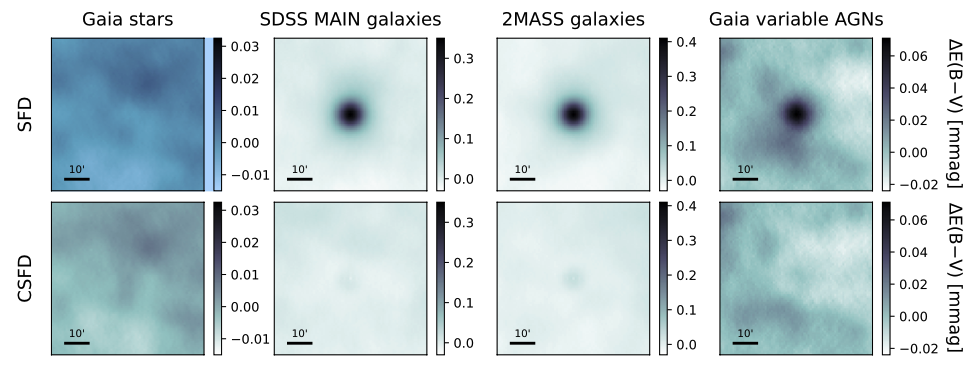
\includegraphics[width=0.7\textwidth]{figures_update2/CSFD_figure7.png}
\caption{Stacked images of the SFD $E(B-V)$ (top row) and the CSFD equivalent (bottom row) centered on different types of sources. From left to right, the stacks are centered on Gaia stars, SDSS main sample galaxies, 2MASS galaxies, and Gaia AGNs, respectively. Aside from the stars, the SFD $E(B-V)$ values around all galaxy samples are biased high due to the LSS contamination. This bias is significantly reduced in CSFD. (Caption and figure adapted from \cite{2023ApJ...958..118C}.)}
\label{default}
\end{center}
\end{figure}

\subsection{Dust as a supernova systematic}

As we all know, intergalactic dust introduces significant scatter to Type Ia supernova (SN Ia) distance estimates. According to \cite{2023arXiv231112098R}, dust is the second-largest source of uncertainty in SNe Type Ia cosmological parameter constraints, accounting for 11.5\% of the total variance. Current SNe analyses include intergalactic dust reddening as a function of wavelength and SN redshift in the systematic error budget, but because the magnitude of the effect is somewhat uncertain, do not correct the distance measures themselves. My COSMOS-Web colleague, Nao Suzuki, pointed out that if we can differentiate extinction laws according to foreground galaxy properties, as we appear to do, then we could derive a more precise calibration for foreground reddening of supernovae. So, our work could have quite high impact. 

\subsection{Bonus: cluster duster}
%Copypasta from AAG
As you all know, I am heavily involved in SuperBIT galaxy cluster gravitational lensing analysis. The methods we use to study circumgalactic dust 
also allow us to gain a ``stratospheric perspective'' on intracluster dust, which is known to trace intracluster light and provide a significant source of cooling in the ICM \cite{2022Univ....8..212S}. Inspired by the analysis of the GUViCS study of dust in the Virgo cluster \cite{2020A&A...633L...7L} which used only 12,000 background galaxies, we will cross-correlate excess reddening of background galaxies with SuperBIT galaxy cluster members, obtaining results qualitatively similar to Figure \ref{fig:clusterdust}. This would be a lot of fun to try out at some point... 

\begin{figure}[htb]\label{fig:clusterdust}
   \centering
   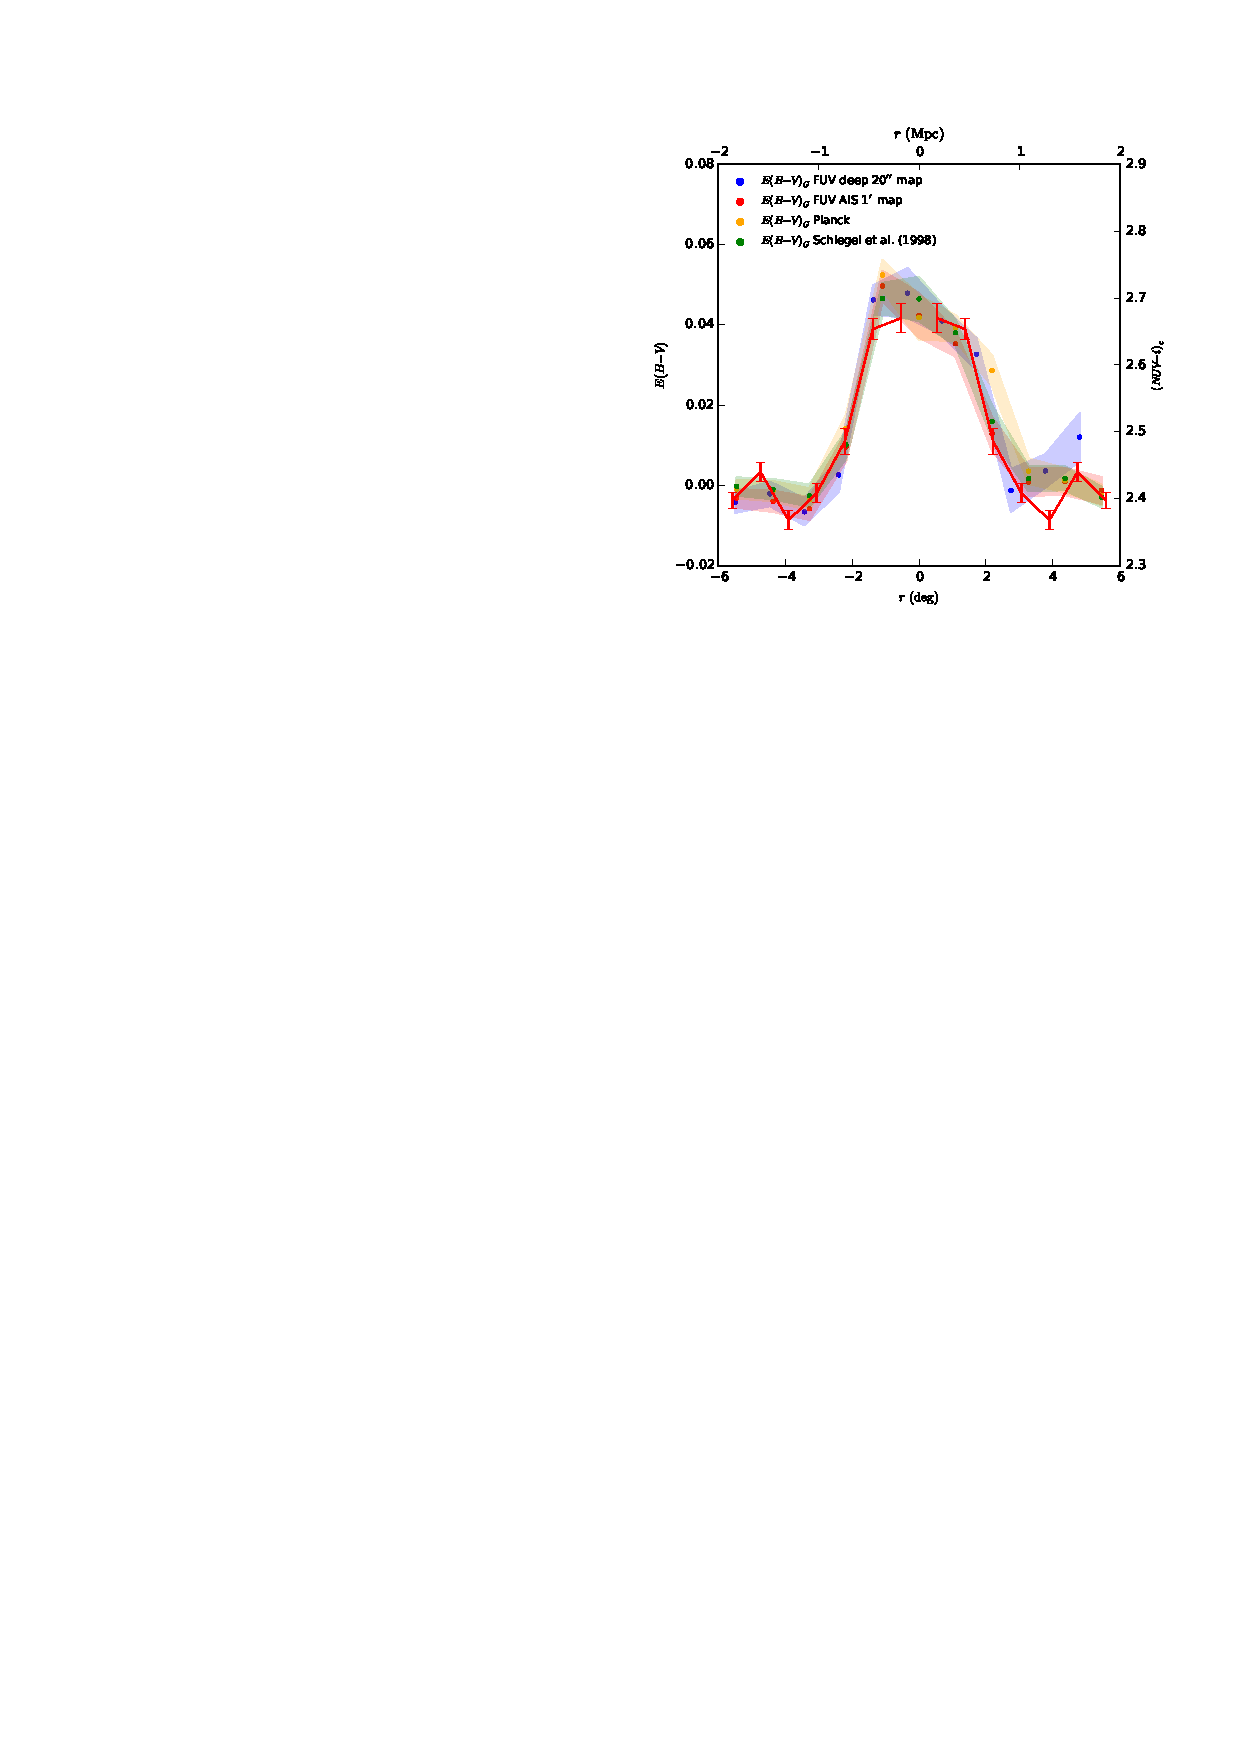
\includegraphics[width=0.5\linewidth]{figures_update2/aa37024-19-fig1.pdf} 
   \caption{Radial profiles of ($NUV-i$) color and $E(B-V)$ for the Virgo cluster. Different colors indicate different foreground extinction schemes. The continuous red line traces the radial extinction profile of Virgo's intracluster dust. From \cite{2020A&A...633L...7L}}
   \label{fig:clusterdust}
\end{figure}



%%%%%%%%%%%%%%%%%%%%%%%%%%%%%%%%%%%
%%%%%%%
%%%%%%% CODE AND MODEL UPDATES
%%%%%%%
%%%%%%%%%%%%%%%%%%%%%%%%%%%%%%%%%%%

%
%
\section{Code and Modeling Updates}\label{sec:code}


%%%%
%%%% COLOR-MATCHED RANDOMS
%%%%

\subsection{Code updates}\label{sec:codeupdates}
\subsubsection{Color-matched randoms}
\begin{itemize}
	\item describe algorithm, show nice figure
	\item This didn't significantly affect the result, however.
\end{itemize}

%%%%
%%%% RANDOM CATALOG GENERATION OVERHAUL
%%%%
\subsubsection{Random catalog generation overhaul}
\begin{itemize}
	\item Mention bug of picking healpixels; could even show the bad ra/good ra figures
	\item Also implemented ability to generate catalogs in galactic coordinates, which made sense for the WISExSCOS catalog
	\item Based on the redMaGiC ratio of random galaxies to real galaxies, the random catalogs I create are $\sim 20 \times$ the length of their respective data catalogs. For very large galaxy catalogs like SDSS, generating an equivalent random catalog with almost a billion objects is too much for my HPC to handle. (Or, perhaps my code is inefficient.) So, I added a little script to create multiple smaller catalogs and concatenated them. While not immediately useful, since I don't think we will be publishing the SDSS results, this may be helpful later.
\end{itemize}

%%%%
%%%% RANDOM CATALOG GENERATION OVERHAUL
%%%%
\subsubsection{Treecorr variance and misc. utilities}
\begin{itemize}
	\item Fixed variance! Used patches and compensated estimates
	\item \texttt{RADec\_to\_healpixel}
	\item deredden magnitudes, the script used to incorporate CSFD extinction values into magnitudes.
	%\item fix magnitude (idnr what that is) 
\end{itemize}

%%%%
%%%% 
%%%%
\subsection{Model improvements}

\subsubsection{Gordon 2023 extinction}
The G23 extinction model is available through the \texttt{dust\_extinction} software package \cite{Gordon2024}.\footnote{\url{https://github.com/karllark/dust_extinction}}. Implementing it in the code was very simple and amounted to adding an import statement for this newer \texttt{dust\_extinction} package in the \texttt{src/extinction\_model.py}. Both G23 and the older CCM89 models are available in \texttt{dust\_extinction}; the \texttt{extinction} Python package is still imported in case someone wants to see results with other old models: Calzetti00, odonnell94, fitz99. As before, the default $R_V$ is 3.1 but any reasonable value is available. 


\subsubsection{CSFD}

As mentioned earlier, Nao pointed me to this CSFD paper \cite{2023ApJ...958..118C}. Since the amplitude of the residual seemed non-negligible ($10^{-4}$) it was worth implementing. I located a nice software package called \texttt{dustmapper}\footnote{\url{https://github.com/gregreen/dustmaps}} to query the CSFD dust map and obtain extinction coefficients for a given set of coordinates. Specifically, there is a handy \texttt{dustmaps.csfd.CSFDQuery} method that takes as input an RA, Dec list in SkyCoords format and returns an array of E(B-V) values. An $R_V$ value is used to convert those into extinction coefficients and then used to de-redden SDSS and DES magnitudes. Using SFD maps to obtain E(B-V), then apply band-specific extinction coefficients to get extinction values.
Subtracting these extinction values A$_{\rm X,\, CSFD}$ from the observed magnitudes \texttt{MAG\_X} to obtain the dereddened magnitudes:
\begin{verbatim}
MAG_X_CORRECTED_CSFD = MAG_X - A_X_CSFD
\end{verbatim}

For the DES magnitudes, I used the corrected magnitude prescription of Pandey et al.~2021, replacing $A_{X,\mathrm{SFD98}}$ with the equivalent CSFD: 
\begin{verbatim}
MAG_X_CORRECTED_CSFD = MOF_CM_MAG + DELTA_MAG_Y4 + DELTA_MAG_CHROM - A_X_CSFD
\end{verbatim}
These magnitude corrections are implemented in \texttt{src/deredden\_magnitudes.py} and \\
\texttt{src/deredden\_sdss\_magnitudes.py}; the important parts of the algorithm are shown in Appendix \ref{appx:deredden}. 

As one might expect, the switch to CSFD had a notable effect on the amplitude of the signal and varied by sample type. For the WISExSuperCOSMOS foreground, CSFD had the effect of decreasing signal amplitude at large impact parameters. For the redMaGiC LRG sample, it had the effect of increasing the extinction at high impact parameters. Details can be found in $\S$\ref{sec:csfdvsnot}.  

\begin{comment}
% Dereddening workflow 
Load up some coordinates in SkyCoords format
Get E(B-V) for those galaxies with dustmap package.
Multiply that  E(B-V) value by RV to get an AV: 0.302*3.1 = 0.9331  
Use dust_extinction to get the A(X)/A(V) extinction curve as I have always done…
Multiply extinction curve A(X)/A(V) by the AV I calculated to get AX
Subtract the AX from magnitudes to get de-reddened magnitudes!
\end{comment}

\subsubsection{Weighted least-squares fitting to profiles.}

To fit models to our results and facilitate comparison to the literature, I have added a function (\texttt{do\_WLS\_fit.py}) to perform weighted least-squares fits to extinction profiles. Surprisingly, we hadn't implemented this yet! The function, partially reproduced in Appendix \ref{appd:wls}, is principally a wrapper for the StatsModel package's weighted least-squares method, with the additional capability to rescale weights for fits in logarithmic space (i.e., power laws). This code was used to generate all fits shown in this report, and weights are based on TreeCorr's estimates of the variance at each point in the extinction profile. 
%Options exist for both logarithmic (i.e., power law) and non-logarithmic (regular, linear bins) fits


%%%%%%%%%%%%%%%%%%%%%%%%%%%%%%%%%%%
%%%%%%%
%%%%%%% CATALOGS
%%%%%%%
%%%%%%%%%%%%%%%%%%%%%%%%%%%%%%%%%%%

\section{Catalogs: Round 2}\label{sec:catalogs}

In the first update, all results presented were made using the WISExSuperCOSMOS (or WISExSCOS) photometric redshift catalog as a foreground and the Dark Energy Survey redMaGiC catalogs \cite{2016MNRAS.461.1431R} as background catalogs. Since that time, there have been a few minor changes to the way these three catalogs are constructed for our analysis. First, the redshift cut for the foreground WISExSCOS catalog galaxies is now $z < 0.2$ from $z < 0.15$, and I have implemented a $17 < bCalCorr < 21$ to minimize stellar confusion at the faint end. Second, a cut of $z > 0.5$ is placed on the high-density redMaGiC sample to ensure adequate foreground-background separation (the full redshift range is $0.15 < z < 0.65$). As before, I also create a $z < 0.45$ subsample of the high-density redMaGiC catalog to investigate the extended CGM of the redMaGiC luminous red galaxies (LRGs).  
 
For all redMaGiC catalogs, CSFD-corrected magnitudes (\texttt{mof\_cm\_mag\_X\_corr\_csfd}) are added to the joined DES Y3 GOLD-redMaGiC background catalogs and used instead of the \texttt{mof\_cm\_mag\_X} magnitudes used before.
%
As stated in the first update, no random catalog is currently available for the WISExSuperCOSMOS surveym and so I create one myself using the updated algorithm described in Section \ref{sec:codeupdates}. This updated WISExSuperCOSMOS random catalog is created in galactic coordinates to match the original catalog format. 

The final catalog sizes are: 1,293,547 galaxies in the southern sky WISExSuperCOSMOS catalog; 871,556 galaxies at $z > 0.5$ in the high-density background redMaGiC catalog; 34,711,359 objects in the $z > 0.5$ high-density background redMaGiC random catalog; 816,204 galaxies in the high-luminosity high-redshift background redMaGiC catalog; 32,597,284 objects in the high-luminosity high-redshift background redMaGiC random catalog; 660,074 galaxies in the foreground $z < 0.45$ high-density redMaGiC catalog; and 26,306,402 galaxies in the foreground $z < 0.45$ redMaGiC catalog. 

The redMaGiC catalogs are downloaded as-is. To add photometry to these catalogs, I apply the following query to the DES Y3 GOLD catalog: 
\begin{verbatim}
SELECT 
  coadd_object_id, ra, dec, l, b, ebv_sfd98, ebv_lenz17, 
  ebv_planck13, a_sed_sfd98_g, a_sed_sfd98_i, a_sed_sfd98_r, 
  a_sed_sfd98_z, a_fiducial_g, a_fiducial_i, a_fiducial_r, a_fiducial_z,
  dnf_zmean_mof, dnf_zmc_mof, delta_mag_y4_g, delta_mag_y4_r, 
  delta_mag_y4_i, delta_mag_y4_z, delta_mag_chrom_g, 
  delta_mag_chrom_r, delta_mag_chrom_i, delta_mag_chrom_z, 
  mof_cm_mag_err_g, mof_cm_mag_err_r, mof_cm_mag_err_i, 
  mof_cm_mag_err_z, mof_cm_mag_g, mof_cm_mag_r, 
  mof_cm_mag_i, mof_cm_mag_z, mof_cm_mag_corrected_g, 
  mof_cm_mag_corrected_r, mof_cm_mag_corrected_i, mof_cm_mag_corrected_z 
  
FROM 
  des_y3_gold_v2_2_c 
  
WHERE 
  flags_footprint = 1 
  AND flags_foreground = 0 
  AND (flags_gold & 1111110) = 0 
  AND (flags_badregions& 110) = 0 
  AND extended_class_mash_mof = 3

\end{verbatim}

\subsection{SDSS and GWSLC}

For the first time in this project, I have expanded our analysis to galaxies in the Northern hemisphere. As originally proposed in the ADAP, the northern background galaxy sample is drawn from the Sloan Digital Sky Survey Data Release 18 catalog. The Sloan Digital Sky survey covers... and after masking to match the WISExSuperCOSMOS catalog, contains an impressive 16,839,045 galaxies. Similar to the DES Y3 catalog used in the Southern sky, the CSFD magnitude correction procedure described above is used to create new magnitude columns.
%From AAG

The query for selecting the background SDSS catalog is based on examples available at CasJobs and follows:

\begin{verbatim}
SELECT 
  g.objid, g.run, g.ra, g.dec, z.z AS redshift, 
  g.u, g.g, g.r, g.i, g.z, g.err_u, g.err_g, g.err_r, g.err_i, g.err_z, 
  g.dered_u, g.dered_g, g.dered_r, g.dered_i, g.dered_z, 
  g.extinction_u, g.extinction_r, g.extinction_i, g.extinction_z,
  g.expRad_r, g.mRrCc_r, g.mRrCcErr_r INTO mydb.sdss_bg_photoz 
  
FROM 
  Galaxy AS g
  JOIN Photoz AS z ON g.objID = z.objID
  
WHERE
  (g.htmid*37 & 0x000000000000FFFF) < (650 * 99)
  AND 
  ((g.flags_r & 0x10000000) != 0)  
  AND
  ((g.flags_r & 0x8100000c00a0) = 0)  
  AND
  (((g.flags_r & 0x400000000000) = 0) OR (g.psfmagerr_r <= 0.3))  
  AND
  (((g.flags_r & 0x100000000000) = 0) OR (g.flags_r & 0x1000) = 0)   
  AND
    (z.z > 0.5)
\end{verbatim}

The WISExSuperCOSMOS catalog covers the whole sky and thus the SDSS area, so that was the first foreground sample constructed for analysis with the SDSS background galaxy catalog. After masking, 1,708,255 WISExSuperCOSMOS galaxies are used as a Northern sky foreground catalog. 

As I was interested in examining the relationship between dust and galaxy properties, I also created a foreground catalog from the GALEX-WISE-SDSS Legacy Catalog (GSWLC), which has physical properties for almost 660,000 galaxies at redshifts $0.01 < z < 0.3$.\footnote{https://salims.pages.iu.edu/gswlc/} Several GSWLC variants are available; this analysis uses the GSWLC-X2, which combines the deepest areas of the GSWLC-A, M and D catalogs and covers 90\% of the SDSS area \cite{2016ApJS..227....2S}. The GSWLC-X2 also features more accurate star formation rates than the first generation of the catalog thanks to joint UV, optical, and mid-IR SED fitting \cite{2018ApJ...859...11S}). The full GSWLC-X2 contains 659,229 galaxies; as recommended by the authors, we restrict our analysis to the 610,518 that are included in the Sloan Digital Sky Survey main galaxy sample (\texttt{flag\_mgs = 1}, see Figure \ref{fig:gwslc}). After masking and a redshift cut at $z < 0.18$ to ensure adequate foreground-background separation, the GSWLC catalog used in this analysis contains 550,060 galaxies. A different subset of the SDSS catalog was created as a background catalog for GWSLC with a total of 18,452,187 galaxies. 

\begin{figure}
\begin{center}
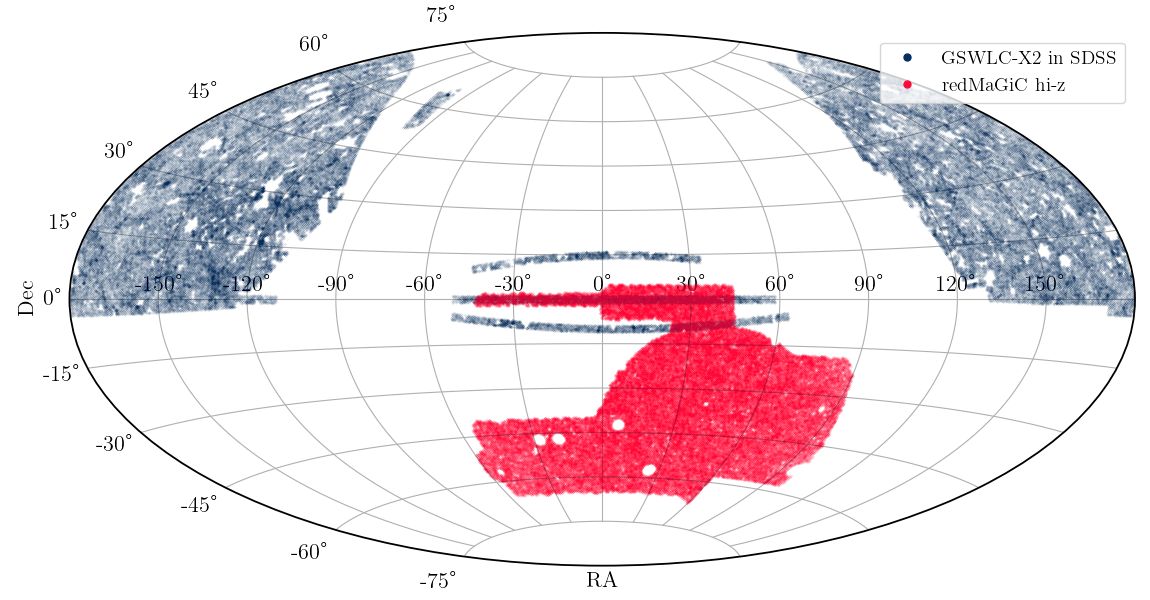
\includegraphics[width=0.75\textwidth]{figures_update2/GSWLC-X2_redmagic_overlap_aitoff.png}
\caption{Sky coverage of redMaGiC high-luminosity high-redshift galaxy sample(red points) and GALEX-WISE-SDSS Legacy Catalog sources in the SDSS main galaxy sample (blue points).}
\label{fig:gwslc}
\end{center}
\end{figure}

Random galaxy catalogs do not seem to be available for either GSWLC-2 or SDSS and so are created using the updated algorithm described in Section \ref{sec:codeupdates}. The random SDSS catalog has 247,369,950 objects; the random GWSLC catalog contains 167,257,476 objects; and the Northern sky random WISExSuperCOSMOS catalog has 5,865,639 objects. 



\subsection{Star catalogs for systematics testing}
Beyond new galaxy catalogs, since update \#1 I have also constructed star catalogs to test for systematics in the analysis. The rationale for using star catalogs is thus: unless embedded in a star-forming region, stars do not have extended halos of dust (certainly not at megaparsec scales!) and so using star catalogs as foreground samples the extinction calculation offers a valuable null test. For the redMaGiC-based catalogs, star catalogs are taken from the Gaia Data Release 3 database \cite{2023A&A...674A...1G}; as before, overlapping regions are obtained by calculating the intersection of masks for each survey of interest. As the Gaia collaboration does not make a survey mask readily available, I create one using a simple function (\texttt{radec2healpixels}) described in Section \ref{sec:code:healpix}. The result for the Gaia stars is shown in Figure \ref{fig:gaiaoverlap}. (Incidentally, the same procedure is carried out to make masks for SDSS and GSWLC). 

Figure \ref{fig:gaiaoverlap} also illustrates the gradient in the number density of stars across the DES field of view approaching the galactic plane. In theory, failing to account for this variation in source density in random catalogs might bias the resulting correlation measurement. As such, both ``signal'' and ``random'' star catalogs are independent, random subsamples of the full Gaia Data Release 3 catalog.

\subsubsection{Gaia stars}
\begin{itemize}
\item This was used as a foreground sample for the redMaGiC catalogs, so it got used for correlations twice: once for the high-density sample, once for the high-luminosity high-redshift sample.   %Editor's note, I have no idea what this means. Maybe because I did redMaGic both samples
\item I had an oddly tough time narrowing down the survey area on Cosmohub, so I ended up grabbing a fairly large area over the Southern sky and applying the redMaGiC mask. Final count: 478,494 objects.
\item Detail catalog cuts, which I don't even remember!
\item Show one of my pretty overlap plots! 
\end{itemize}

\begin{figure}[htbp]
\begin{center}
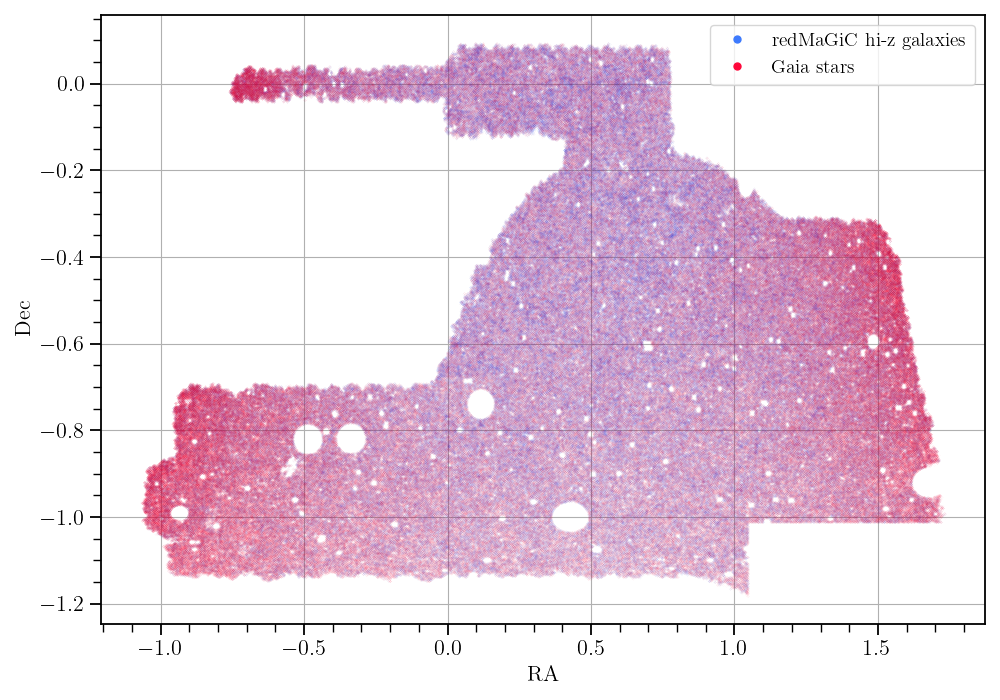
\includegraphics[width=0.75\textwidth]{figures_update2/masked_gaia_rmz_hiz_overlap_rectilin.png}
\caption{default}
\label{fig:staroverlap}
\end{center}
\end{figure}

\begin{comment}
COMMENT SELECT `designation`, `solution_id`, `source_id`, `random_index`, `ref_e
COMMENT poch`, `ra`, `dec`, `bp_rp`, `bp_g`, `g_rp`, `l`, `b`, `ecl_lon`, `ecl_l
COMMENT at`, `in_qso_candidates`, `in_galaxy_candidates`, `non_single_star` FROM
COMMENT  gaia_dr3_source WHERE ACOS( SIN(RADIANS(`dec`)) * SIN(RADIANS(-30)) + C
COMMENT OS(RADIANS(`dec`)) * COS(RADIANS(-33)) * COS(ABS(RADIANS(`ra`) - RADIANS
COMMENT (50))) )*180/PI() &lt;= 100   
\end{comment}

\subsubsection{DES Y3 stars}
\begin{itemize}
\item This was used as a background sample, standing in for the redMaGiC catalogs in a correlation with WISExSuperCOSMOS 
\item Show catalog query used, which was taken from \cite{2021ApJS..254...24S}.
\item Detail catalog cuts made, which include $18 < \rm{mag\_r\_corr} < 21$. 
\item After masking and the like, there were 824,345 stars in the ``real'' catalog and 9,892,452 randoms. 
\end{itemize}

\begin{comment}
COMMENT SELECT `coadd_object_id`, `ra`, `dec`, `l`, `b`, `ebv_sfd98`, `ebv_lenz1
COMMENT 7`, `ebv_planck13`, `a_sed_sfd98_g`, `a_sed_sfd98_i`, `a_sed_sfd98_r`, `
COMMENT a_sed_sfd98_z`, `a_fiducial_g`, `a_fiducial_i`, `a_fiducial_r`, `a_fiduc
COMMENT ial_z`, `dnf_zmean_mof`, `dnf_zmc_mof`, `delta_mag_y4_g`, `delta_mag_y4_
COMMENT r`, `delta_mag_y4_i`, `delta_mag_y4_z`, `delta_mag_chrom_g`, `delta_mag_
COMMENT chrom_r`, `delta_mag_chrom_i`, `delta_mag_chrom_z`, `mof_cm_mag_err_g`, 
COMMENT `mof_cm_mag_err_r`, `mof_cm_mag_err_i`, `mof_cm_mag_err_z`, `mof_cm_mag_
COMMENT g`, `mof_cm_mag_r`, `mof_cm_mag_i`, `mof_cm_mag_z`, `mof_cm_mag_correcte
COMMENT d_g`, `mof_cm_mag_corrected_r`, `mof_cm_mag_corrected_i`, `mof_cm_mag_co
COMMENT rrected_z` FROM des_y3_gold_v2_2_c                                      
COMMENT WHERE FLAGS_FOOTPRINT = 1 AND FLAGS_FOREGROUND = 0 AND (FLAGS_GOLD &amp;
COMMENT  1111100) = 0 AND (EXTENDED_CLASS_MASH_MOF &lt;= 2) AND (MOF_PSF_MAG_R +
COMMENT  DELTA_MAG_Y4_R + DELTA_MAG_CHROM_R - A_SED_SFD98_R &gt; 16) AND (MOF_PS
COMMENT F_MAG_R + DELTA_MAG_Y4_R + DELTA_MAG_CHROM_R - A_SED_SFD98_R &lt; 23)   
\end{comment}

%%%%%%%%%%%%%%%%%%%%%%%%%%%%%%%%%%%
%%%%%%%
%%%%%%% RESULTS
%%%%%%%
%%%%%%%%%%%%%%%%%%%%%%%%%%%%%%%%%%%

\section{Results}\label{sec:results}


\begin{itemize}
\item Comments for the individual samples are below, but globally, both the SFD and CSFD results agrees with the \textit{exponent} of the \cite{2010MNRAS.406.1815M} power law (Equation 13 in that reference) within one sigma. However, the \textit{amplitude} of the CSFD relationship is twice as high as the \cite{2010MNRAS.406.1815M} result. I am not entirely sure what to make of this, but it is what it is. 
\item Could discuss the SFD results...
\end{itemize}

\subsection{RedMaGiC-based results}\label{sec:redmagic_results}

\begin{figure}[htb]
\begin{center}

\includegraphics[width=0.75\textwidth]{figures_update2/dustcorrel_redmagic_csfd_newrand_withfits.png}
\caption{Extinction vs impact parameter for WISExSuperCOSMOS (blue points) and redMaGiC LRGs (maroon points). Power-law fits are shown for the redMaGiC LRG profile (maroon dashed line) and the combined WISExSuperCOSMOS x redMaGiC profiles (blue dashed line). For comparison, the M10 result is shown in red. Results are based on the CSFD Milky Way extinction correction.}
\label{fig:redmagicfits}
\end{center}
\end{figure}


\subsubsection{WISExSuperCOSMOS foreground}

The extinction profiles of WISExSuperCOSMOS galaxies as measured with redMaGiC background galaxies are shown in Figure \ref{fig:redmagicfits}: the result from cross-correlation with the $z > 0.5$ high-density redMaGiC sample is shown in dark blue; the result from cross-correlation with the high-redshift redMaGiC sample is shown in light blue. In both cases, the extinction profiles follow a broken power law, with a rapid decrease from $A_V \sim 0.3$ to $A_V \sim 0.02$ in the inner 50 kpc \hinv, then a slower decline to $A_V \sim 0.02$ at 1 Mpc \hinv . At the transition to the 2-halo regime ($r \gtrsim 2$ Mpc \hinv), the extinction profiles rapidly diminish to below our detection threshold ($A_V \sim 10^{-5}$). 

I fit power laws to the WISExSuperCOSMOS extinction profiles in the 1-halo regime (50 kpc \hinv $ < r < 1$ Mpc \hinv); the inner limit is set to the point where the redMaGiC LRG extinction and WISExSuperCOSMOS profiles intersect, and the outer limit to the points where the extinction begins to roll off. 

The best-fit power law to the extinction profile obtained with the $z > 0.5$ high-density redMaGiC sample is given by Equation \ref{eqn:hidens}: 
% Equation 1
\begin{equation}
A_V(r) = \left(1.14 \pm 0.08\right) \times 10^{-2} \left( \frac{r}{h^{-1}\, \mathrm{kpc}} \right)^{-0.84 \pm 0.04}\label{eqn:hidens}
\end{equation}

Similarly, for the extinction profile obtained with the $z > 0.5$ high-lum high-$z$ redMaGiC sample is given by Equation \ref{eqn:hiz}:
% Equation 2
\begin{equation}
A_V(r) = \left(1.02 \pm 0.11\right) \times 10^{-2} \left( \frac{r}{h^{-1}\, \mathrm{kpc}} \right)^{-0.72 \pm 0.06}\label{eqn:hiz}
\end{equation}

Combining the two WISExSuperCOSMOS $\times$ redMaGiC profiles, the best fit power law is Equation \ref{eqn:stacked}; this is the result I plan to publish.  
% Equation 3
\begin{equation}
A_V(r) = \left(1.08 \pm 0.07\right) \times 10^{-2} \left( \frac{r}{h^{-1}\, {\rm kpc}} \right)^{-0.77 \pm 0.04}\label{eqn:stacked}
\end{equation}



\subsubsection{redMaGiC LRG}

Cross-correlation of the redMaGiC LRG galaxy sample ($z < 0.45$ high-density redMaGiC) with the redMaGiC high-lum high-$z$ sample produced the extinction curve shown in Figure \ref{fig:redmagicfits}. As might be expected for this foreground population, there is little apparent extinction at the lowest impact parameters ($r < 50$ kpc \hinv). While qualitatively similar to the SuperCOMSOS-based results in the one-halo regime, the LRG sample shows significant extinction well into the two-halo regime. The best-fit power law to this profile is given by Equation \ref{eqn:lrg}:

\begin{equation}
A_V(r) = \left(0.82 \pm 0.19\right) \times 10^{-2} \left( \frac{r}{h^{-1}\, \mathrm{kpc}} \right)^{-0.69 \pm 0.06}\label{eqn:lrg}
\end{equation}

The exponent and amplitude of Equation \ref{eqn:lrg} agree with the combined redMaGiC fit of Equation \ref{eqn:stacked} to within about 1 $\sigma$ through the one-halo regime ($r \lesssim 1 Mpc$).  

\subsubsection{Comparison to SFD}\label{sec:csfdvsnot}

Given the acknowledged problems of SFD98, the CSFD formulation is the default Milky Way extinction correction employed in this work. It may still be of interest to compare the profiles obtained with the SFD and CSFD prescriptions; this is shown for the three redMaGiC-based profiles in Figure \ref{fig:csfdvsnot}. I noticed a couple of interesting trends here. First, there didn't seem to be much of an effect for the high-density background catalog, but using the SFD extinction correction, the high-lum high-z profile has more extinction at high impact parameters. Put differently, it appears that the SFD prescription added too much extinction at high impact parameters, and with CSFD the two redMaGiC catalogs produce consistent results for WISExSuperCOSMOS. On the other hand, compared to the SFD98 prescription, the CSFD prescription added a significant amount of dust at higher impact parameters for the redMaGIC LRG sample, leading to significant reddening past 1 Mpc \hinv. Although quite different from the effect for the WISExSuperCOSMOS result, this behavior for LRG is consistent with the idea that SFD98 overcorrected foreground extinction due to contamination from the LSS. If one assumes that the LRG is a particularly biased tracer of the LSS, then it makes sense that the CSFD prescription adds some reddening back in. 

\begin{figure}[htb]
\begin{center}

\includegraphics[width=\textwidth]{figures_update2/dustcorrel_redmagic_csfd_vs_not_all.png}
\caption{Comparison of extinction profiles obtained with the SFD98 Milky Way reddening correction (light blue) and CSFD (medium blue). From left to right, profiles are shown for WISExSuperCOSMOS galaxies cross-correlated with high-density redMaGiC background galaxies, for WISExSuperCOSMOS galaxies cross-correlated with high-luminosity high-redshift redMaGiC background galaxies, and for high-density redMaGiC galaxies cross-correlated with high-luminosity high-redshift redMaGiC background galaxies. The M10 profile is plotted in red.}
\label{fig:csfdvsnot}
\end{center}
\end{figure}

For the sake of comparison, I also fit power laws to extinction profiles resulting from the SFD98 Milky Way foreground prescription. The best-fit power law to the extinction profile obtained with the $z > 0.5$ high-density redMaGiC sample is given by Equation \ref{eqn:hidenssfd}: 

% Equation 1
\begin{equation}
A_V(r) = \left(5.9 \pm 2.3\right) \times 10^{-3} \left( \frac{r}{h^{-1}\, \mathrm{kpc}} \right)^{-0.62 \pm 0.12}\label{eqn:hidenssfd}
\end{equation}

The best-fit power law to the extinction profile obtained with the high-lum high-$z$ redMaGiC sample is given by Equation \ref{eqn:hizsfd}: 
% Equation 2
\begin{equation}
A_V(r) = \left(9.5 \pm 0.9\right) \times 10^{-3} \left( \frac{r}{h^{-1}\, \mathrm{kpc}} \right)^{-0.75 \pm 0.03}\label{eqn:hizsfd}
\end{equation}

The result of a fit to the combined WISExSuperCOSMOS x redMaGIC profiles is
% Equation 3
\begin{equation}
A_V(r) = \left(8.7 \pm 1.3\right) \times 10^{-3} \left( \frac{r}{h^{-1}\, \mathrm{kpc}} \right)^{-0.74 \pm 0.08}\label{eqn:stackedsfd}
\end{equation}

As above, Equations \ref{eqn:hidenssfd}--\ref{eqn:stackedsfd} describe the flatter parts of the profiles (50 kpc \hinv $ < r < 1$ Mpc \hinv). 
Finally, the SFD98-based LRG profile is best fit by Equation \ref{eqn:lrgsfd}
% Equation 4
\begin{equation}
A_V(r) = \left(6.9 \pm 2.1\right) \times 10^{-3} \left( \frac{r}{h^{-1}\, \mathrm{kpc}} \right)^{-0.87 \pm 0.14}\label{eqn:lrgsfd}
\end{equation}

For this last profile, my WLS algorithm just would not produce a reasonable fit, which forced me to adopt a conventional least-squares algorithm for the LRG fit. The prefactor of Equation \ref{eqn:lrgsfd} matches the fit of Equation \ref{eqn:lrg} within error bars, however, the exponents are in a 3 $\sigma$ disagreement. Meanwhile, the fits of Equations \ref{eqn:hidenssfd}--\ref{eqn:stackedsfd} agree with \ref{eqn:hidens}--\ref{eqn:stacked} within 1 $\sigma$.



\subsection{Systematics testing results}\label{sec:systematics_results}

This section summarizes the results of the systematics tests described in Section \ref{sec:catalogs}, namely, the calculation of extinction profiles using star catalogs as either foreground or background samples (Figures \ref{fig:systematics}). The CSFD Milky Way reddening correction was implemented for all fits, and except where noted, the WLS algorithm was used to calculate fits to the extinction profiles. Overall, these fits are consistent with zero, with amplitudes and exponents on the order of $10^{-4}$. 

\textbf{Note}: I decided to tabulate the systematics test results rather than format them like the power laws of $\S$ \ref{sec:results} because I didn't want to distract from our main results. Happy to change it if you think it would be better. 


\begin{table}[htp]
\caption{Fit results for star-based extinction profiles}
\begin{center}
\begin{tabular}{|c|c|c|}
\hline
\textbf{Sample} & \textbf{Prefactor} & \textbf{Exponent} ($\ee{-5}$)\\
\hline
Gaia \x redMaGiC high-density & $1.0\, \pm \, (3.6 \ee{-4})$ &  
$-6.7 \, \pm$  8.9\\
Gaia \x redMaGiC high-$z$ & $1.0\, \pm \, (2.9 \ee{-4})$ & 
$1.1 \, \pm \, 7.6$\\
Gaia \x redMaGiC combined & $1.0\, \pm \, (2.1 \ee{-4}$) &
$-2.1 \pm 5.6$\\
WISExSCOS \x DES stars & $1.0 \, \pm \, (1.1 \ee{-3}$) & 
$-3.2\, \pm \, 47$ \\
\hline
\end{tabular}
\end{center}
\label{tab:systematics}
\end{table}%


The top row of Figure \ref{fig:systematics} shows the the extinction profile resulting from the cross-correlation of the Gaia star foreground catalog with the redMaGiC high-luminosity high-redshift sample (maroon points) and high-density sample (red points). The left panel shows the full impact parameter range; the right panel is cropped to show values at higher impact parameters. 

%Excluding the first two points, which seemed to skew the fits, 
The exponents and prefactors of best-fit power laws to these two profiles, plus the fit to the stacked redMaGiC profiles, are tabulated in the first three rows of Table \ref{tab:systematics}. The best-fit power law to the stacked high-dens and high-lum high-z profiles is overplotted in Figure \ref{fig:systematics} as a medium-red dashed line. In all fits, the amplitude is consistent with 1 and the exponent is one ten-thousandth of the size of the signal (!). This result sounds incredible, but the full fit printout in $\S$\ref{appx:gaiafg} seems to back up the assertion. So, this is a strong confirmation of the validity of our results. 

\begin{figure}[htb]
\begin{center}
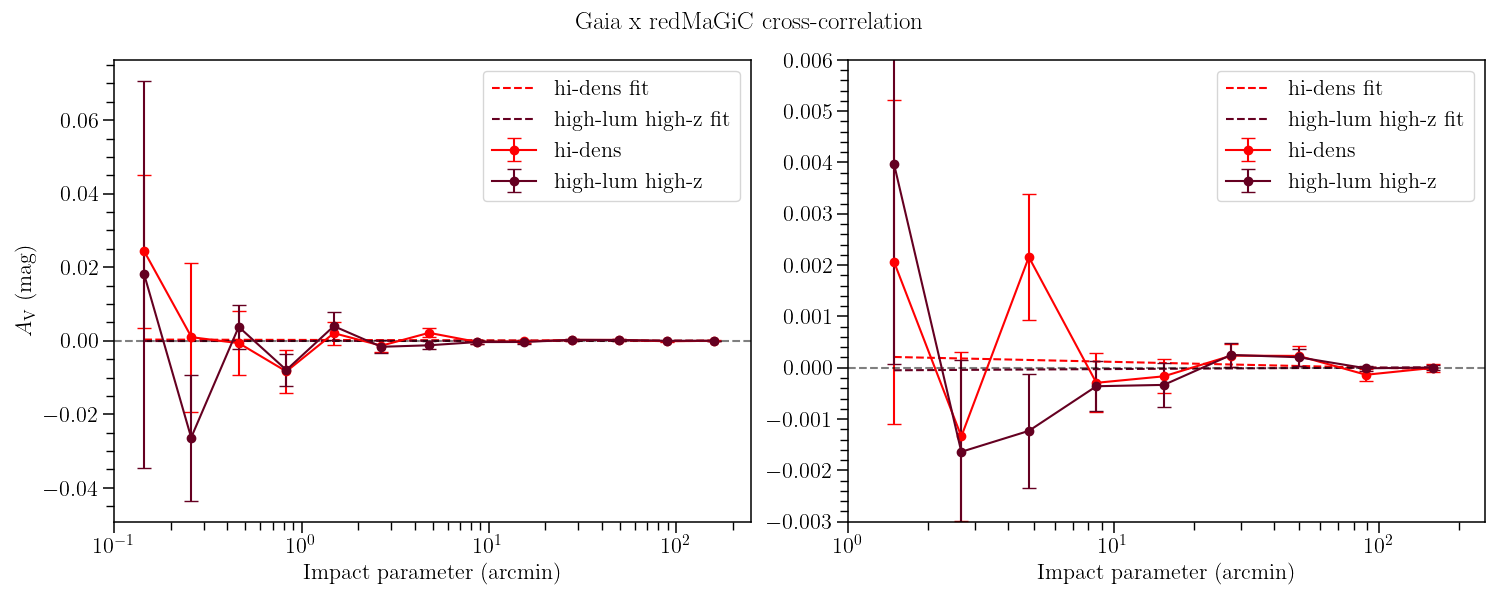
\includegraphics[width=0.95\linewidth]{figures_update2/Gaia_redmagic_crosscorrel_csfd.png}\\
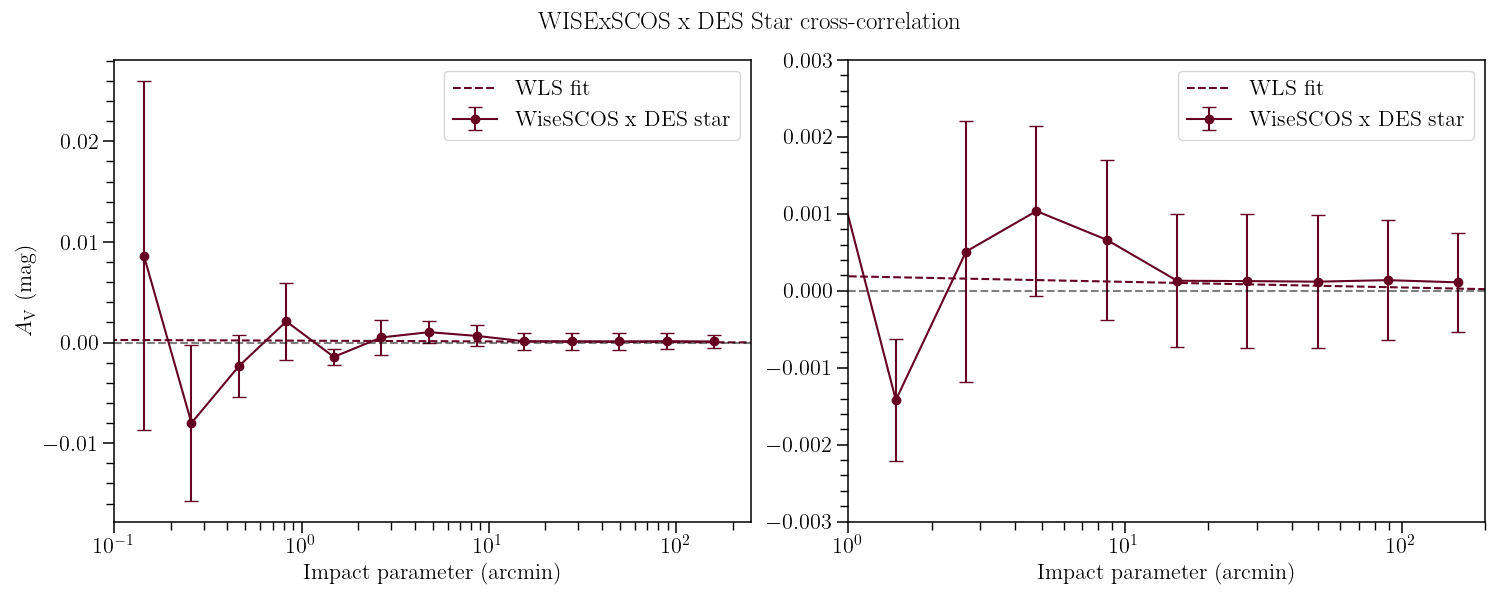
\includegraphics[width=0.95\linewidth]{figures_update2/desstar_crosscorrel_csfd.png}
\caption{Top panels: Gaia star foreground catalog cross-correlated with redMaGiC high-luminosity high-redshift (maroon) and high-density (red) background catalogs. The best-fit power law to the stacked redMaGiC-based profiles is plotted as a dark red dashed line. Bottom panels: WISExSuperCOSMOS foreground cross-correlated with DES Y3 stars. Left panels shows the full range of impact parameters considered; right panels show values at higher impact parameters only.} 
\label{fig:systematics}
\end{center}
\end{figure}

Similarly, the bottom row of Figure \ref{fig:systematics} shows the \av profile resulting from the cross-correlation of the WISExSuperCOSMOS foreground with the background catalog created from DES Y3 stars (see $\S$\ref{sec:catalogs} for details). The best-fit power law to this profile is overplotted as a dashed maroon line and the parameters of this fit are tabulated in the bottom row of Table \ref{tab:systematics}. Note that for this particular fit, I decided to use the result of an unweighted least-squares result, not the WLS used elsewhere. The justification is essentially aesthetic: while the WLS fit yielded an exponent essentially consistent with zero ($1.78 \ee{-4} \pm 1.28 \ee{-4}$), the exponent was ten times larger than exponents from the WLS-based Gaia foreground fits, which in turn made the DES background \av plots look far worse than they were. Meanwhile, the LSQ fits yielded a much smaller value, albeit with a large error bar ($-3.15 \ee{-5} \pm 4.71 \ee{-4}$). Regardless, even in the pessimistic case of the WLS, the OOM of the exponent is less than one-thousandth of the OOM of the galaxy \av profiles. The WLS and regular LSQ fits are compared below, and the full WLS fit results may be found in Appendix \ref{appx:desfit}.  

%% I may have skipped the first two points? And these are certainly
%% based on the updated galactic-coord randoms. 
\begin{verbatim}
WISExSCOS x DES star WLS fit results:
  Coeff: -5.348e-04 +/- 4.500e-04
  Slope: 1.770e-04 +/- 1.284e-04

WISExSCOS x DES Y3 stars LSQ:
  Const: 1.878e-04 +/- 1.265e-03
  Slope: -3.150e-05 +/- 4.713e-04
\end{verbatim}


\subsection{BONUS: SDSS-based results}\label{sec:sdss}

These results are based on two separate foreground catalogs: the same WISExSuperCOSMOS catalog used for the southern sky and the GWSLC catalog described above. I will go through these results separately. These are certainly interesting to see because so far we hadn't extended the search to the Northern sky. However, these results probably aren't publication-ready: the WISExSCOS \x SDSS \av profile doesn't fall off with distance but flattens out, and while the GSWLC \x SDSS profile is actually a pretty decent match to the other profiles at low and high impact parameters, there is an odd dip at the middle that depends on the NSIDE of the mask. 

That said, may be an argument to be made for publishing just \textit{low} impact parameter points. Those points consistently line up quite well with the redMaGiC-based results at these impact parameters, and Eric did note the significance of the detection of extended dust halos in what is really the extended CGM. But, we can discuss this.

\subsubsection{WISExSuperCOSMOS x SDSS}
The \av profile resulting from cross-correlation of the WISExSuperCOSMOS foreground catalog with an SDSS catalog is shown in Figure \ref{fig:sdss}. I had really wanted this one to work, since this is the same foreground sample we use elsewhere that gave us successful results. And at impact parameters of less than 100 kpc \hinv (2-3 arcminutes), the profile qualitatively matches the redMaGiC-background \av profiles of Figure \ref{fig:redmagicfits}. However, that fat tail past 3 arcminutes is the stickiest result of all of my results. Color cuts on the background galaxies, aggressive masking, etc. do nothing. I had even hoped that CSFD, which is supposedly a superior extinction correction algorithm, would make it go away, but all to no avail. 

\begin{figure}[htbp] %  figure placement: here, top, bottom, or page
  \centering
  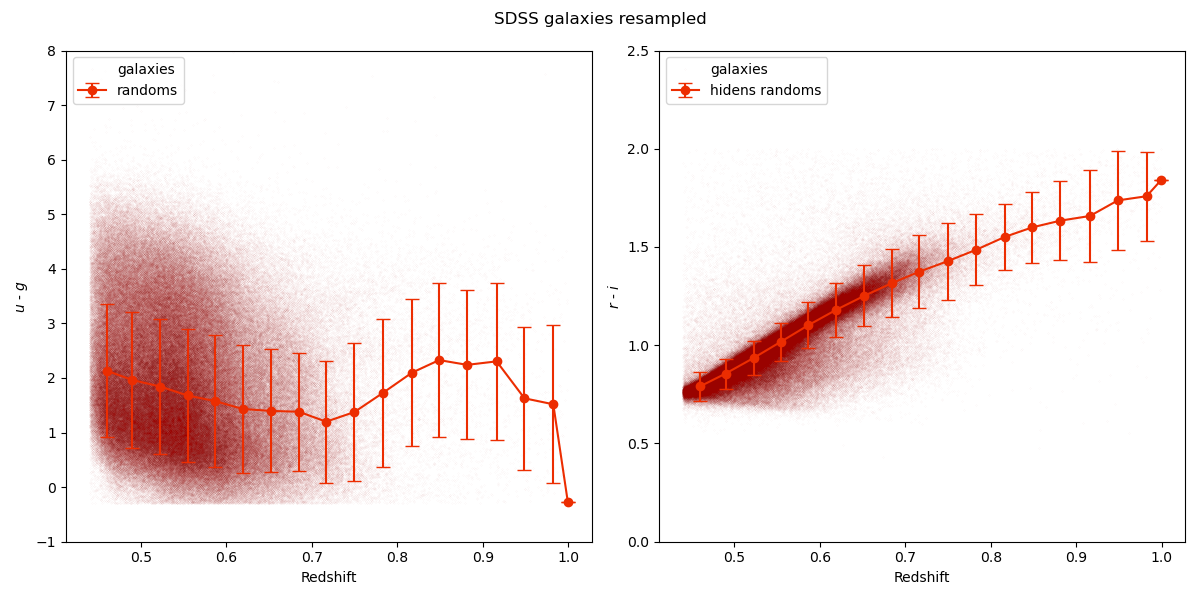
\includegraphics[width=0.8\linewidth]{
  	figures_update2/color_redshift_sdss_lrg_resamp2.png}\\ 
  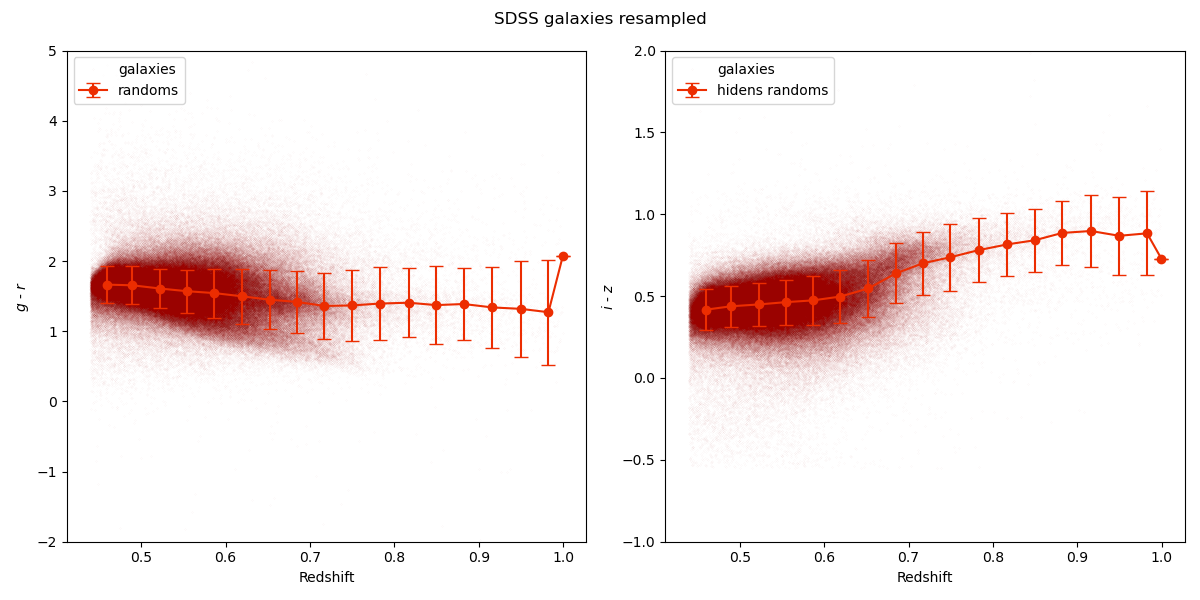
\includegraphics[width=0.8\linewidth]{
  	figures_update2/color_redshift_sdss_lrg_resamp1.png}\\ 	
   \caption{Color-redshift diagrams of the SDSS galaxy and random catalogs used in this analysis. Real galaxies are shown as small, dark red points. The mean value of random galaxies created for this analysis are shown as larger, bright red points.}
   \label{fig:sdsscolorredshift}
\end{figure}

Figure \ref{fig:sdsscolorredshift} shows the color-redshift space of the SDSS galaxies used in this analysis, as well as the color-redshift of the random catalogs I created following the procedure outlined above. Even with quality cuts and an $i - z > -0.103$ selection, the color space is clearly quite complicated. Since what characterizes the redMaGiC sample is tightness in color space, I also tried to use the \href{https://www.sdss4.org/science/final-bao-and-rsd-measurements/}{eBOSS LRG sample}. Unfortunately, the source density was too low to be used: 377,458 galaxies in LRG sample spread out over tens of thousands of square degrees. So, the results (with the SFD98 extinction!) didn't look like much. 

\begin{figure}[htb]
\begin{center}
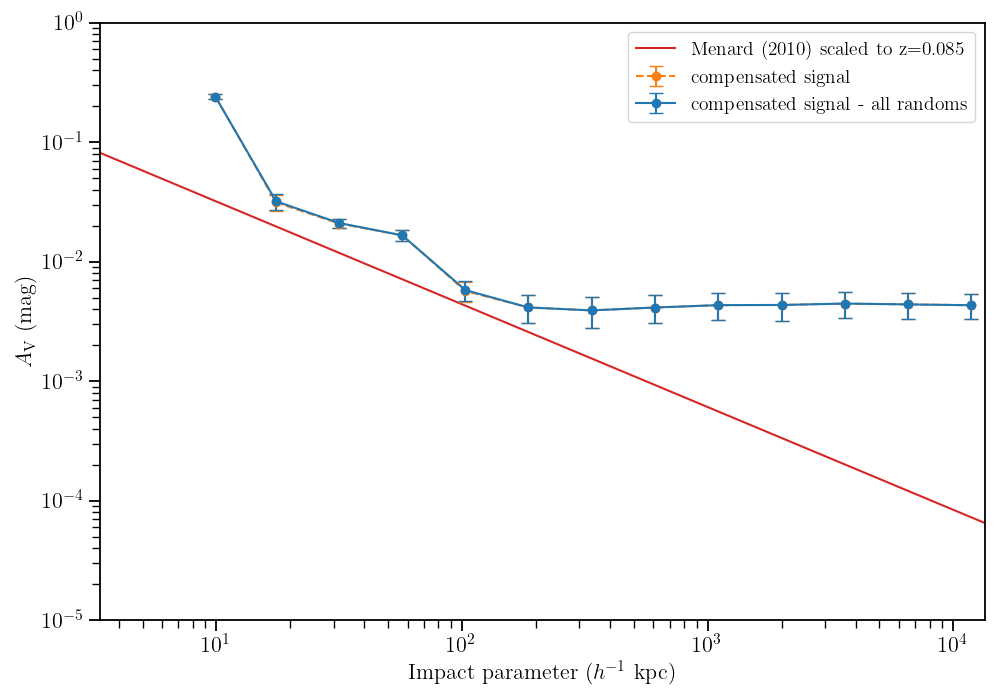
\includegraphics[width=0.65\linewidth]{figures_update2/compensated_dustcorrel_csfd_4zbins_figure.png}
\caption{Extinction curve for WISExSuperCOSMOS foreground galaxies cross-correlated with SDSS background galaxies (blue points) with all randoms subtracted. The ``compensated'' profile produced by TreeCorr is shown in orange. The M10 profile is shown in red.} 
\label{fig:sdss}
\end{center}
\end{figure}

\subsubsection{GSWLC x SDSS}
As discussed above, I also tried to get a fit with GSWLC-X2, since that catalog has star-formation information and would allow us to assess the difference in dust halos between quiescent and star-forming galaxies. The resulting \av for the GSWLC-X2 foreground catalog cross-correlated with a color-cut SDSS catalog is shown in red in Figure \ref{fig:uglycolor}. 

I find this result to be quite interesting: at low impact parameters (r $<$ 50 kpc \hinv) \textit{and} at high impact parameter/the two-halo regime (r $>$ 1 Mpc \hinv), the \av profile lines up very nicely with the redMaGiC samples, with an amplitude somewhere between redMaGiC LRG and WISExSuperCOSMOS. However, that dip in the middle is somewhat mysterious to me. Its exact location also seems to depend heavily on the NSIDE of the HEALPix mask I create for the catalog. his is a possible indication of my mask being incomplete or wrong; this is why I don't 100\% trust the result. For the sake of completeness, I decided to fit a power law to the outermost six points of this GSWLC \x SDSS extinction profile, with the result shown in Equation \ref{eqn:gwslc}:

\begin{equation}
A_V(r) = \left(1.5 \pm 0.4\right) \times 10^{-2} \left( \frac{r}{h^{-1}\, \mathrm{kpc}} \right)^{-0.76 \pm 0.07}\label{eqn:gwslc}
\end{equation}

As one might expect from Figure \ref{fig:uglycolor}, this relationship agrees very nicely with Equations \ref{eqn:stacked} and \ref{eqn:lrg}.

\textbf{Quiescent vs. star-forming dust profiles}. Around May of 2024, I experimented with calculating extinction profiles on GWSLC-X2 data segregated by specific star formation rates (sSFR). I was very curious to see the difference in \av between quiescent galaxies, defined by the GSWLC group as having $\log_{10}(\mathrm{sSFR} < -11.5 $ in the M or D GSWLC UV sub-sample, and star-forming galaxies with $\log_{10}(\mathrm{sSFR} > -11.5$ in any GSWLC UV sub-sample.\footnote{https://salims.pages.iu.edu/gswlc/}. With a cut at $z < 0.2$, there were about 187,000 quiescent galaxies and 208,000 actively star-forming galaxies (Figure \ref{fig:gswlcMstarHist}). The results are shown in Appendix \ref{appx:gwslc} and Figure \ref{fig:gswlcMstarHist} in particular. While cool, Figure \ref{fig:gswlcMstarHist} left me a little bemused, particularly the large dip in the middle of the profiles. Moreover, the selection functions and sky coverage are also quite heterogenous between the quiescent and star-forming samples, which surely complicates the interpretation of the result. As an additional caveat, these results are based on the out-of-date SFD98 correction, as the CSFD Milky Way extinction correction scheme had not yet been implemented in the code. Since I wasn't even sure I understood the whole GWSLC sample result, redoing this complicated quiescent versus star-forming analysis didn't seem worth it. But complications aside, this is an interesting line of inquiry, so we can pick it up again after submission. 

\begin{figure}[htb]
\begin{center}

\includegraphics[width=0.49\linewidth]{figures_update2/dustcorrel_gwslc_csfd_withfit.png}

\includegraphics[width=0.49\linewidth]{figures_update2/dustcorrel_all_csfd_withfit_uglycolor.png}

\caption{Extinction curve resulting from cross-correlation of GSWLC foreground and SDSS background galaxies. The GSWLC-SDSS result is shown in isolation in the left panel in red and together with the redMaGiC-based results in the right panel: WISExSuperCOSMOS--high-luminosity high-redshift (blue), WISExSuperCOSMOS--high density (orange), and the redMaGiC LRG fit (green). The M10 profile is plotted in black in both panels.} 
\label{fig:uglycolor}
\end{center}
\end{figure}


Spatial overlap plot: put this into catalogs. 

\begin{comment}
%% In case I decide to include his figure caption
Taken from Figure 12 of Van Alfen et al. (2024). The position–position (left), positions–orientation (middle), and orientation–orientation (right) correlation functions for both IllustrisTNG300-1 and a galaxy catalog build using halotools. The points with error bars show the correlations from IllustrisTNG300-1 and the solid lines show correlations from a galaxy catalog built using halotools with the Bolshoi-Planck (BolPlanck) halo catalog with our alignment component addition.
\end{comment}


%%%%%%%%%%%%%%%%%%%%%%%%%%%%%%%%%%%
%%%%%%%
%%%%%%% DISCUSSION
%%%%%%%
%%%%%%%%%%%%%%%%%%%%%%%%%%%%%%%%%%%

\section{Discussion and Next Steps}\label{sec:discussion}
\subsection{Comment on results}
\begin{itemize}
\item Fact of the matter is that I have been playing with this for years and the results have been consistent.
\item The long time period has afforded me the opportunity to modernize, like 2023 dust relation, CSFD, WLS, etc. 
\item The fact that CSFD is high is consistent with the claim of \cite{2023ApJ...958..118C} that ``when SFD is used to derive absolute photometry for sources, Galactic extinction will be overcorrected in a redshift- and spatially-dependent manner following the pattern of the cosmic web.'' Now, which is more believable is at the reader's discretion! 
\item Also, to some extent, it is to be expected that amplitude of signal is proportional to volume covered in foreground (right?). Then again, volume of M\'{e}nard sample is significantly higher than ours. As far as I know, that study has no selection for red sequence galaxies [Not sure what I meant by this -- ed.] 
\item To end on a bright note, we know that the redMaGiC galaxies are biased tracers of LSS (by biased here I mean have a high galaxy bias relative to some field galaxy). The presence of dust well into the two-halo regime, while the WISExSuperCOSMOS samples (which presumably include star-forming galaxies) fall off, tells a cool story about redMaGiC as a tracer of LSS and WISExSuperCOSMOS a little more general. 
\end{itemize}

\subsection{Next steps}
\begin{itemize}
\item At this point, I would like to publish. One can fiddle with results ad infinitum, but I've been urged by multiple people to publish so I will. If you all want to start running systematic analyses, you can, but I am not going to wait around.  
\item I figure this is a beginning, not an end. In follow-on studies, we can do calibration, segregate by galaxy type, etc. (Note that I had tried to do a galaxy type study (motivation for SDSS/GWSLC!) but my results were inconclusive and I haven't redone them since.) 
\item For northern-sky samples, it might be worth trying Pan-STARRS instead of SDSS, or perhaps KiDS or some other such thing. I don't know what the benefits would be of a more ``modern'' survey over SDSS, but it would be interesting to see. 
\item At some point, I would also like to selecting a foreground catalog from the Galaxy and Mass Assembly (GAMA) catalog, which in DR4 provides stellar mass, morphological classification, and  other physical characteristics for over 330,000 galaxies across four regions of the sky (G09, G12, G15, and G23) totaling 250 deg$^2$ \cite{2011MNRAS.413..971D, 2022MNRAS.513..439D}. 

\item Jim, still waiting on your emission study! Also, Eric, could we transfer ownership of main repository to me? Alternatively, I can sync my fork.
\item My ultimate goal is to make a function or tool that can help calibrate SN extinction along the line of sight as a function of impact parameter. 
\item Cluster duster! Copy and paste from my AAG, but this would be an extremely fun result. 
\end{itemize}


%%%%%%%%%%%%%%%%%%%%%%%%%%%%%%%%%%%
%%%%%%%
%%%%%%% APPENDIX
%%%%%%%
%%%%%%%%%%%%%%%%%%%%%%%%%%%%%%%%%%%

\newpage
\appendix 

\section{Appendix: Dereddening code}\label{appx:deredden}
This is the key part of the magnitude de-reddening code \texttt{src/deredden\_magnitudes.py}. 

\begin{verbatim}

    cat = fits.open(catname, mode='update', save_backup=True)
    ra = cat[1].data['ra']
    dec = cat[1].data['dec']
    coords = SkyCoord(ra, dec, frame='icrs', unit='deg')
    print("Got catalog, coordinates")

    # Get our E(B-V) values
    csfd = CSFDQuery()
    ebv = csfd(coords)
    print("Queried coordinates")

    # Convert to Av values
    Rv = 3.1
    Av_values = ebv * Rv

    # Do dust modeling
    gordon23 = G23(Rv=Rv)
    AxAv = gordon23.evaluate(wavelengths, Rv)

    # Finally, calculate offsets. np.newaxis makes it a column vector
    Ax = Av_values[:, np.newaxis] * AxAv
    Ax = Ax.T 
    print("Obtained Ax for catalog")

    # OK, time to do corrected magnitudes
    data = cat[1].data

    # First, define bandpass column names in catalog
    band_names = [`u', `g', `r', `i', `z']

    # Let's go through band by band and add these column names
    print("Beginning magnitude corrections...")
    corr_band_dict = {}

    for i in range(len(band_names)):

        # Do actual correction
        this_Ax = Ax[i,:]
        corr_band = data[band_names[i]] - this_Ax

        # Define a key name, extend dict with it
        key_name = f'{band_names[i]}_corr_csfd'
        corr_band_dict[key_name] = corr_band

    # Now make this an HDU, write to file
    print(f"Adding new magnitude columns to catalog {catname}")
    columns = data.columns
    for key, value in corr_band_dict.items():
        try:
            col = fits.Column(name=key,  format=`D', array=value)
            columns.add_col(col)
        except ValueError:
            pass
\end{verbatim}

\section{Appendix: Weighted least-squares fit and results}\label{appd:wls}

The important parts of \texttt{do\_WLS\_fit.py} are reproduced below. 

\small

\begin{verbatim}
	import statsmodels.api as sm
	import numpy as np
	
def do_WLS_fit(this_dk, dust_rel, name=None, start=None, end=None, log=False):
    """
    Perform a weighted least-squares linear regression to
    data, taking care to transform the variables appropriately.

    Inputs
        this_dk: should be the `compensated' treecorr output
        dust_rel: the corrected A_V relationship (dk-dr+rr)
        name: what are we calling it?
        start: exclude points with index < 'start' for fitting
        end: ibidem, but for points with index > 'end'
        log: if True, fit the relationship in log-space to stabilize the fits.
             Default is False.
    """
    
    ## If you want to exclude some points at the start/end 
    dust_rel = dust_rel[start:end]
    this_dk = this_dk[start:end]
    
    ## If doing a logarithmic fit, transform the 
    ## dependent variable (the fully compensated TreeCorr kappa)
    if log == True:
        # Keep positive values only
        ok = (dust_rel > 0)
        dust_rel = dust_rel[ok]
        this_dk = this_dk[ok]
        
        # Fitting log of dust relation, so take log
        Y = np.log(dust_rel)
        
        ## Also need to transform the weights!
        weights_OG = 1/(this_dk[`sigma']**2)
        #weight_scale = (1/Y)**2
        weight_scale = (1/(Y+1))**2
        weights = weights_OG * weight_scale
    
    ## If not doing a logarithmic fit, don't transform
    else:
        Y = dust_rel
        weights = 1/(this_dk[`sigma']**2)
    
    ## If plotting X on a log-scale, which we are, 
    ## fit relationship on log scale
    X = this_dk['meanlogr']

    ## Add intercept to abscissa
    X = sm.add_constant(X)

    ## Do fit
    mod_wls = sm.WLS(Y, X, weights=weights)
    res_wls = mod_wls.fit()

    ## Print results
    print("")
    print(f"Fit result: {name}")
    print("")
    print(res_wls.summary())

    return(res_wls)\end{verbatim}

\normalsize 

\section{Full weighted least-squares regression results}

Full printouts of the \texttt{statsmodels.api.WLS} regressions are reproduced below. For real fits (not the systematics tests), the constant term is converted to a coefficient as $e ^ {\rm const}$ in the power law. 

\subsection{WISExSCOS and redMaGiC fits}

The fit results below are based on only the ``flat'' portions of the extinction curves in Figure \ref{fig:redmagicfits}, i.e., 50-1000 kpc for the CSFD fits, and results are based on a high-redshift subset ($z_{\rm redmagic} > 0.5$) of the redMaGiC high-density catalog.  

\small 
\begin{verbatim}
                            WLS Regression Results                            
==============================================================================
Dep. Variable:                      y   R-squared:                       0.975
Model:                            WLS   Adj. R-squared:                  0.973
Method:                 Least Squares   F-statistic:                     397.0
Date:                Wed, 23 Oct 2024   Prob (F-statistic):           2.23e-09
Time:                        18:59:41   Log-Likelihood:                 8.2589
No. Observations:                  12   AIC:                            -12.52
Df Residuals:                      10   BIC:                            -11.55
Df Model:                           1                                         
Covariance Type:            nonrobust                                         
==============================================================================
                 coef    std err          t      P>|t|      [0.025      0.975]
------------------------------------------------------------------------------
const         -4.5308      0.068    -66.556      0.000      -4.683      -4.379
x1            -0.7677      0.039    -19.925      0.000      -0.853      -0.682
==============================================================================
Omnibus:                        1.628   Durbin-Watson:                   2.041
Prob(Omnibus):                  0.443   Jarque-Bera (JB):                1.154
Skew:                          -0.692   Prob(JB):                        0.562
Kurtosis:                       2.373   Cond. No.                         6.06
==============================================================================

Notes:
[1] Standard Errors assume that the covariance matrix of the errors is correctly specified.
[-4.53082712 -0.7676558 ]
Fit: 1.08e-02 * (meanr)^-0.77
\end{verbatim}
\normalsize

Below is the full fit result for the redMaGiC LRG sample, i.e., the low-redshift subset ($z_{\rm redmagic} > 0.5$) of the redMaGiC high-density sample cross-correlated with the high-luminosity high-redshift 

\small
\begin{verbatim}

Fit result: redmagic LRG

                            WLS Regression Results                            
==============================================================================
Dep. Variable:                      y   R-squared:                       0.943
Model:                            WLS   Adj. R-squared:                  0.936
Method:                 Least Squares   F-statistic:                     148.0
Date:                Wed, 23 Oct 2024   Prob (F-statistic):           6.85e-07
Time:                        18:59:41   Log-Likelihood:                -2.4161
No. Observations:                  11   AIC:                             8.832
Df Residuals:                       9   BIC:                             9.628
Df Model:                           1                                         
Covariance Type:            nonrobust                                         
==============================================================================
                 coef    std err          t      P>|t|      [0.025      0.975]
------------------------------------------------------------------------------
const         -4.8020      0.225    -21.318      0.000      -5.312      -4.292
x1            -0.6872      0.056    -12.166      0.000      -0.815      -0.559
==============================================================================
Omnibus:                        7.605   Durbin-Watson:                   1.874
Prob(Omnibus):                  0.022   Jarque-Bera (JB):                3.122
Skew:                          -1.072   Prob(JB):                        0.210
Kurtosis:                       4.487   Cond. No.                         13.8
==============================================================================

Notes:
[1] Standard Errors assume that the covariance matrix of the errors is correctly specified.
[-4.80200583 -0.68720111]

Fit: 8.21e-03 * (meanr)^-0.69

\end{verbatim}
\normalsize

\subsection{Gaia x redMaGiC}\label{appx:gaiafg}

Gaia foreground cross-correlated with redMaGiC high-luminosity high-redshift sample. 
\small 
\begin{verbatim}
Fit result: Gaia x hi-lum hi-z

                            WLS Regression Results                            
==============================================================================
Dep. Variable:                      y   R-squared:                       0.002
Model:                            WLS   Adj. R-squared:                 -0.089
Method:                 Least Squares   F-statistic:                   0.02226
Date:                Wed, 23 Oct 2024   Prob (F-statistic):              0.884
Time:                        18:48:14   Log-Likelihood:                 70.136
No. Observations:                  13   AIC:                            -136.3
Df Residuals:                      11   BIC:                            -135.1
Df Model:                           1                                         
Covariance Type:            nonrobust                                         
==============================================================================
                 coef    std err          t      P>|t|      [0.025      0.975]
------------------------------------------------------------------------------
const      -3.676e-05      0.000     -0.102      0.920      -0.001       0.001
x1          1.133e-05   7.59e-05      0.149      0.884      -0.000       0.000
==============================================================================
Omnibus:                        0.812   Durbin-Watson:                   2.270
Prob(Omnibus):                  0.666   Jarque-Bera (JB):                0.628
Skew:                           0.015   Prob(JB):                        0.730
Kurtosis:                       1.923   Cond. No.                         51.2
==============================================================================
\end{verbatim}
\normalsize

Gaia foreground cross-correlated with redMaGiC high-density sample.

\small 
\begin{verbatim}

Fit result: Gaia x high-dens

                            WLS Regression Results                            
==============================================================================
Dep. Variable:                      y   R-squared:                       0.049
Model:                            WLS   Adj. R-squared:                 -0.037
Method:                 Least Squares   F-statistic:                    0.5696
Date:                Wed, 23 Oct 2024   Prob (F-statistic):              0.466
Time:                        18:48:14   Log-Likelihood:                 69.030
No. Observations:                  13   AIC:                            -134.1
Df Residuals:                      11   BIC:                            -132.9
Df Model:                           1                                         
Covariance Type:            nonrobust                                         
==============================================================================
                 coef    std err          t      P>|t|      [0.025      0.975]
------------------------------------------------------------------------------
const          0.0003      0.000      0.740      0.475      -0.001       0.001
x1          -6.73e-05   8.92e-05     -0.755      0.466      -0.000       0.000
==============================================================================
Omnibus:                        0.378   Durbin-Watson:                   3.063
Prob(Omnibus):                  0.828   Jarque-Bera (JB):                0.490
Skew:                          -0.175   Prob(JB):                        0.783
Kurtosis:                       2.115   Cond. No.                         36.3
==============================================================================

\end{verbatim}
\normalsize

Finally, Gaia foreground cross-correlated with the combined redMaGiC galaxy sample.
 
\small 
\begin{verbatim}
Fit result: Gaia x combined redMaGiC

                            WLS Regression Results                            
==============================================================================
Dep. Variable:                      y   R-squared:                       0.006
Model:                            WLS   Adj. R-squared:                 -0.035
Method:                 Least Squares   F-statistic:                    0.1458
Date:                Wed, 02 Oct 2024   Prob (F-statistic):              0.706
Time:                        18:24:35   Log-Likelihood:                 138.85
No. Observations:                  26   AIC:                            -273.7
Df Residuals:                      24   BIC:                            -271.2
Df Model:                           1                                         
Covariance Type:            nonrobust                                         
==============================================================================
                 coef    std err          t      P>|t|      [0.025      0.975]
------------------------------------------------------------------------------
const          0.0001      0.000      0.422      0.677      -0.000       0.001
x1         -2.139e-05    5.6e-05     -0.382      0.706      -0.000    9.42e-05
==============================================================================
Omnibus:                        1.496   Durbin-Watson:                   2.023
Prob(Omnibus):                  0.473   Jarque-Bera (JB):                0.966
Skew:                          -0.059   Prob(JB):                        0.617
Kurtosis:                       2.063   Cond. No.                         45.5
==============================================================================

Notes:
[1] Standard Errors assume that the covariance matrix of the errors is correctly specified.
[ 1.11602366e-04 -2.13928514e-05]

Gaia x combined redMaGiC WLS fit:
  Const: 1.116e-04 +/- 2.646e-04
  exponent: -2.139e-05 +/- 5.603e-05
\end{verbatim}
\normalsize 

\subsection{WISExSuperCOSMOS x DES stars}\label{appx:desfit}

Standard WISExSuperCOSMOS foreground sample cross-correlated with DES Y3 star sample background. The \texttt{rand2} refers to the new random-catalog generation algorithm I used, which 

\small 
\begin{verbatim}
Fit result: WISExSCOS x DES star

                            WLS Regression Results                            
==============================================================================
Dep. Variable:                      y   R-squared:                       0.147
Model:                            WLS   Adj. R-squared:                  0.070
Method:                 Least Squares   F-statistic:                     1.900
Date:                Wed, 02 Oct 2024   Prob (F-statistic):              0.195
Time:                        18:24:36   Log-Likelihood:                 69.816
No. Observations:                  13   AIC:                            -135.6
Df Residuals:                      11   BIC:                            -134.5
Df Model:                           1                                         
Covariance Type:            nonrobust                                         
==============================================================================
                 coef    std err          t      P>|t|      [0.025      0.975]
------------------------------------------------------------------------------
const         -0.0005      0.000     -1.188      0.260      -0.002       0.000
x1             0.0002      0.000      1.378      0.195      -0.000       0.000
==============================================================================
Omnibus:                        0.407   Durbin-Watson:                   1.947
Prob(Omnibus):                  0.816   Jarque-Bera (JB):                0.509
Skew:                          -0.268   Prob(JB):                        0.775
Kurtosis:                       2.193   Cond. No.                         7.93
==============================================================================

Notes:
[1] Standard Errors assume that the covariance matrix of the errors is correctly specified.
[-0.00053476  0.000177  ]

WISExSCOS updated rand x DES star WLS fit results:
  Coeff: -5.348e-04 +/- 4.500e-04
  exponent: 1.770e-04 +/- 1.284e-04
\end{verbatim}
\normalsize 

%%%%%%
%%%%%%
\section{Additional GWSLC results}\label{appx:gwslc}
%%%%%%
%%%%%%

%%%%
\subsection{GWSLC x SDSS fits}\label{appx:GwslcFit}
This is the fit result for a subset of the GWSLC X-2 foreground catalog cross-correlated with a background catalog selected from SDSS. In this case, the fit is based on the six outer points in the profile: $ r > 1 \, {\rm Mpc} \, h^{-1}$. 
%%%% 

\small 
\begin{verbatim}
Fit result: partial GWSLC x SDSS

                            WLS Regression Results                            
==============================================================================
Dep. Variable:                      y   R-squared:                       0.969
Model:                            WLS   Adj. R-squared:                  0.961
Method:                 Least Squares   F-statistic:                     124.3
Date:                Tue, 15 Oct 2024   Prob (F-statistic):           0.000368
Time:                        09:08:29   Log-Likelihood:                0.91149
No. Observations:                   6   AIC:                             2.177
Df Residuals:                       4   BIC:                             1.761
Df Model:                           1                                         
Covariance Type:            nonrobust                                         
==============================================================================
                 coef    std err          t      P>|t|      [0.025      0.975]
------------------------------------------------------------------------------
const         -4.2028      0.264    -15.926      0.000      -4.935      -3.470
x1            -0.7612      0.068    -11.148      0.000      -0.951      -0.572
==============================================================================
Omnibus:                          nan   Durbin-Watson:                   1.677
Prob(Omnibus):                    nan   Jarque-Bera (JB):                0.340
Skew:                           0.319   Prob(JB):                        0.844
Kurtosis:                       2.025   Cond. No.                         10.5
==============================================================================

Notes:
[1] Standard Errors assume that the covariance matrix of the errors is correctly specified.
[-4.20276501 -0.7611631 ]

GWSLC x SDSS Fit:     1.45e-02 * (meanr)^-0.75
partial GWSLC x SDSS Fit:     1.50e-02 * (meanr)^-0.76
\end{verbatim}
\normalsize 


%%%%
\subsection{Algorithm for quiescent/star-forming galaxy separation}
%%%%

\small 
\begin{verbatim}
# Load in GSWLC-X2 catalog with SDSS footprint, initialize comments
cat = Table.read(`GSWLC-X2_in_SDSS.fits')

# Filter out objects with flag_sed !=0 and also do a redshift cut
keep = (cat[`z'] < 0.18) & (cat[`flag_sed'] == 0)
cat = cat[keep]


# Calculate specific star formation rate (sSFR) 
# and elimate those with sSFR == 0
sSFR = np.power(cat[`log_SFRsed'],10) / np.power(cat[`log_M_star'], 10)
nonzero = (sSFR != 0)
cat = cat[nonzero]; sSFR = sSFR[nonzero]

# Add sSFR column column for convenience
cat.add_column(np.log10(sSFR), name='log10_sSFR')

# Select the quiescent galaxies
# These selections are based on Salim et al. 2018 criteria
ok_for_passive = (
    (cat[`UV_survey'] == 2) | (cat[`UV_survey'] == 3)
    ) 
    & (np.log10(sSFR) < -11.5)
passive = cat[ok_for_passive]

# Select star-forming!
star_forming = (np.log10(sSFR) > -11.5)
sf_gals = cat[star_forming]

# Write catalogs to file
passive.write(`gswlc_quiescent_galaxies.fits', overwrite=True)
sf_gals.write(`gswlc_sf_galaxies.fits', overwrite=True)
\end{verbatim}
\normalsize


%%%%
\subsection{Stellar mass and star-forming/quiescent profiles}
%%%%

As a reminder, these are the results of cross-correlating the GSWLC-X2 foreground catalog with the SDSS background galaxy catalog. At low impact parameters, the star-forming galaxies have twice as much extinction as the quiescent galaxies, in line with expectations. At larger impact parameters, the trend is opposite to what one might expect from Figure \ref{fig:redmagicfits}: the quiescent galaxies have little dust, while the star-forming galaxies have dust well into the two-halo regime. Before reading too much into this difference, it should be noted that the SFD98 extinction correction was used for all profiles here. Based on the CSFD vs. SFD98 results shown in Figure \ref{fig:csfdvsnot}, I expect that adopting CSFD would increase the amplitude of the signal for quiescent galaxies and decrease the signal of star-forming galaxies. This will be the subject of future exploration! 

\begin{figure}[htbp] %  figure placement: here, top, bottom, or page
   \centering
   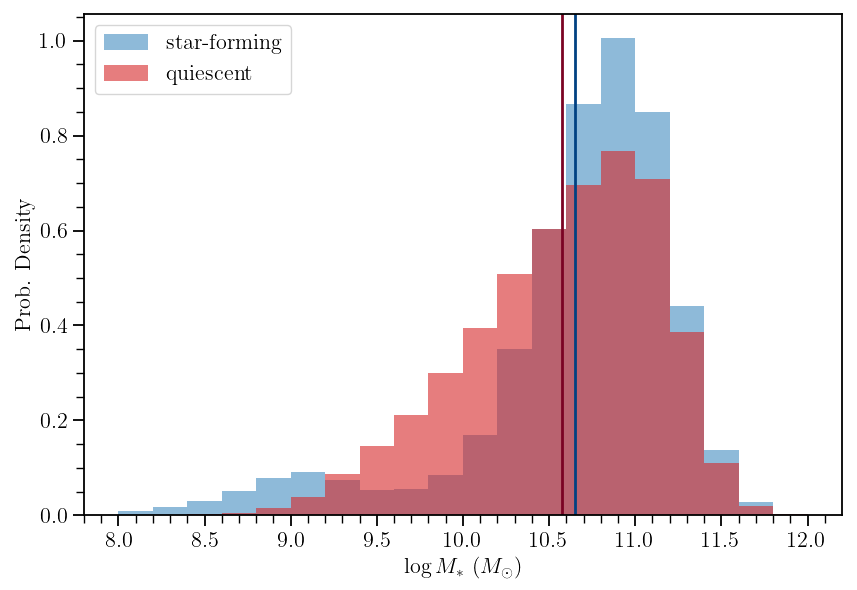
\includegraphics[width=0.65\linewidth]{figures_update2/gswlc_Mstar_hist_withlines.png} 
   \caption{Distribution of stellar masses for quiescent galaxies (red) and star-forming galaxies (blue) selected from the GSWLC-X2 catalog.}
   \label{fig:gswlcMstarHist}
\end{figure}

\begin{figure}[htbp] %  figure placement: here, top, bottom, or page
   \centering
   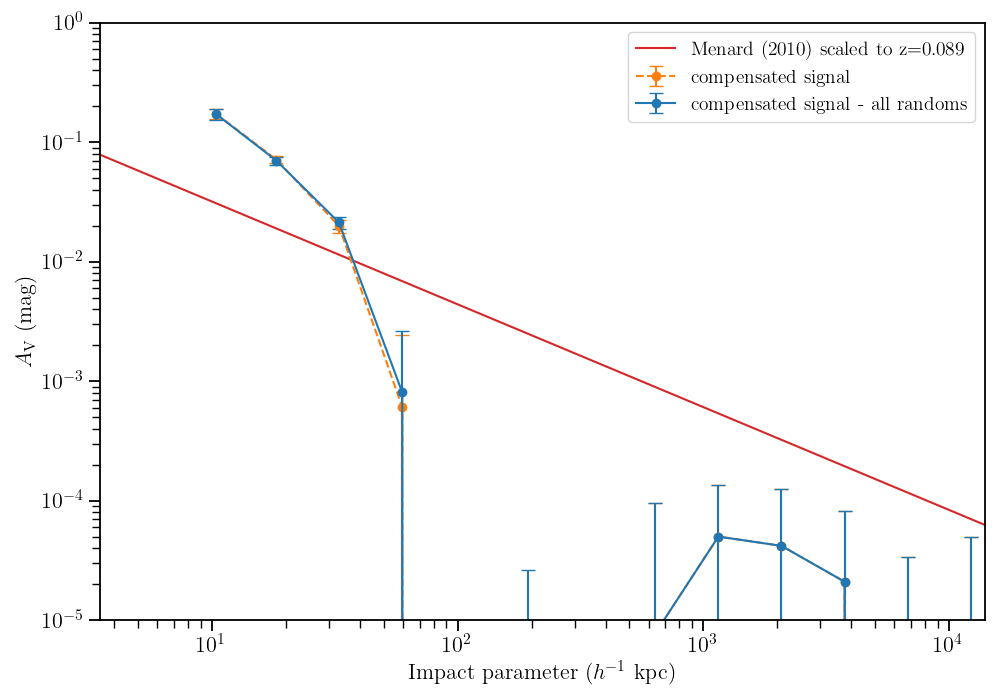
\includegraphics[width=0.49\linewidth]{
   	figures_update2/compensated_dustcorrel_quiescent_10zbins_figure.png
	}
   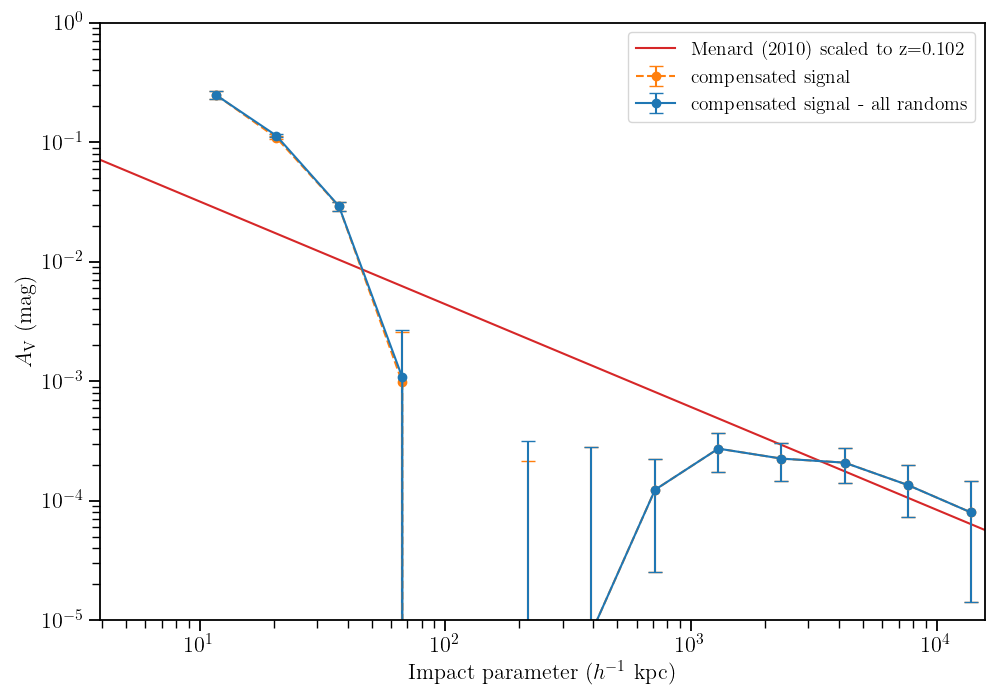
\includegraphics[width=0.49\linewidth]{
	figures_update2/compensated_dustcorrel_sf_10zbins_figure.png
	}  
   \caption{\av profiles for quiescent galaxies (left) and star-forming galaxies (right). Results are based on SFD98 Milky Way extinction correction.}
   \label{fig:GswlcSfQuies}
\end{figure}


%%%%%%%%%%%%%%%%%%%%%%%%%%%%%%%%%%%
%%%%%%%
%%%%%%% BIBLIOGRAPHY
%%%%%%%
%%%%%%%%%%%%%%%%%%%%%%%%%%%%%%%%%%%

\printbibliography

\end{document}  